%!TEX root = paper.tex
\section{Implementation}
\label{sec:implementation}
This section presents our preliminary implementation of InferSpark, which
as a first step, supports a class of Bayesian networks known as the 
exponential-conjugate family. These include the popular LDA model and its
variants. The primary inference algorithm for the exponential-conjugate family
is VMP and thus it's the target of our implementation at present.
In future, the InferSpark language will be extended to support more Bayesian
networks and the appropriate algorithms will be included in our system
as well.

The main jobs of InferSpark are Bayesian network construction and 
code generation (\figref{fig:workflow}). 
%Bayesian network construction first extracts Bayesian network template from the model definition and transforms it into a
%Scala class with inference and query APIs at compile time. 
%Then, code generation takes those as inputs and generates a Spark program
%that can generate the messaging passing graph with VMP on top.
We use the code generation approach because it enables a more flexible API
than a library. For a library, there are fixed number of APIs for user to
provide data, while InferSpark can dynamically generate custom-made APIs 
according to the structure of the Bayesian network. 
Another reason for using code generation is
that compiled programs are always more efficient than interpreted programs.
Afterwards, the generated program would be executed on Spark.
We next describe the implementation of
these modules and our runtime data partition strategies.


%The code generation to implement InferSpark. 
%Stage 1 constructs
%a and submitted to Spark.  
%Stage 2 performs metadata collection using Spark and generate MPG 
%construction and VMP inference code based on the meta data at run time.


%\subsection{Stage 1 Code Generation}
\subsection{Bayesian Network Construction}\label{bnc}

In this offline compilation stage, the model definition is first transformed into a Bayesian network.
We use the macro annotation, a compile-time meta programming facility of
Scala.  It is currently supported via the macroparadise plugin. After the
parser phase, the class annotated with ``{\sf @Model}'' annotation is passed from the
compiler to its transform method. InferSpark treats the class passed to it as
model definition and transforms it into a Bayesian network.

\begin{figure}[!h]
\scriptsize
	\begin{tabular}{lrl}
		ModelDef		& ::= & `@Model' `class' id \\
					&     &`(' ClassParamsOpt `)' `\{' Stmts `\}' \\
		ClassParamsOpt	& ::= & `' /* Empty */ \\
						&	| &	ClassParams \\
		ClassParams		& ::= & ClassParam  [`,' ClassParams] \\
		ClassParam		& ::= & id `:' Type \\
		Type			& ::= & `Long' | `Double' \\
		Stmts			& ::= & Stmt [[semi] Stmts]\\
		Stmt			& ::= & `val' id = Expr \\
		Expr			& ::= & `\{' [Stmts [semi]] Expr `\}' \\
						&	| & DExpr	\\
						&   | & RVExpr \\
						&	| & PlateExpr \\
						&	| & Expr `.' `map' `(' id => Expr `)'\\
		DExpr			& ::= & Literal	\\
						&   | & id \\
						&   | & DExpr (`+' | `-' | `*' | `/') DExpr \\
						&   | & (`+' | `-') DExpr	\\
		RVExpr			& ::= & `Dirichlet' `(' DExpr `,' DExpr `)' \\
						&   | & `Beta' `(' DExpr `)' \\
						&   | & `Categorical' `(' Expr `)' \\
						&   | & RVExpr RVArgList	\\
						&   | & id	\\
		RVArgList		& ::= & `(' RVExpr `)' [ RVArgList ] \\
		PlateExpr		& ::= & DExpr `until' DExpr	\\ 
						&   | & DExpr `to' DExpr	\\
						&	| & `?' \\
						&	| & id
	\end{tabular}
\caption{InferSpark Model Definition Syntax}
\label{fig:inferspark_syntax}
\end{figure}

\figref{fig:inferspark_syntax} shows the syntax of InferSpark model
definition. The expressions in a model definition is divided into 3
categories: deterministic expressions (DExpr), random variable expressions
(RVExpr) and plate expressions. The deterministic expressions include
literals, class parameters and their arithemetic operations. The random
variable expressions define random variables or plates of random variables.
The plate expressions define plate of known size or unknown size. The random
variables defined by an expression can be binded to an identifier by the value
definition. It is also possible for a random variable to be binded to multiple
or no identifiers. To uniquely represent the random variables, we assign
internal names to them instead of using the identifiers.

\begin{figure}[ht]
\centering
	\includegraphics[width=0.6\columnwidth]{figs/two_coins_internal_bn1.eps}
	\caption{Internal Rep. of Bayesian Network}
	\label{fig:two_coins_internal_bn1}
\end{figure}

Internally, InferSpark represents a Bayesian network in a tree form, where the
leaf nodes are random variables and the non-leaf nodes are plates. The edges
in the tree represent the nesting relation between plates or between a plate
and random variables. The conditional dependencies in the Bayesian network are
stored in each node.  The root of the tree is a predefined plate TOPLEVEL with
size 1.  \figref{fig:two_coins_internal_bn1} is the internal representation of
the two-coin model in \figref{fig:two_coins_bn1}, where
$r_1$, $r_2$, $r_3$, $r_4$, correspond to $\pi$, $\phi$, $z$, $x$, respectively. 
Plate 1 and Plate 2 correponds to the plates defined on lines 3--5 in
\figref{fig:two_coins_modeldef}. 

If a plate is nested within another plate,
the inner plate is repeated multiple times, in which case,
the size attribute of the plate node will be computed by summing the size of each
repeated inner plate. We call the size attribute in the tree {\em flattened size}
of a plate. For example, in \figref{fig:two_coins_nestedplates}, the flattened
size of the innermost plate around $x$ is $\sum_i N_i$.

%\begin{figure*}[!h]
%\centering
%\scriptsize
%	\begin{tabular}{|p{0.45\textwidth}|p{0.45\textwidth}|}
%		\hline
%%		ModelDef ::= @Model class id (ClassParamsOpt) \{ Stmts \} & 
%%		\begin{tabular}{l}
%%			env = {}; \\
%%			curPlate = TOPLEVEL;\\
%%			transform(ClassParamsOpt, curPlate, env); \\
%%			transform(Stmts, curPlate, env); \\
%%			genCode(TOPLEVEL, env);
%%		\end{tabular}\\\hline
%%
%%		ClassParams ::= ClassParam [, ClassParams] & 
%%		\begin{tabular}{l}
%%			transform(ClassParam, curPlate, env);\\
%%			transform(ClassParams, curPlate, env);
%%		\end{tabular} \\\hline
%%
%		ClassParam ::= id ':' Type &
%		\begin{tabular}{l}
%			env.push(id, ClassParam(Type))
%		\end{tabular} \\\hline
%%
%%		Stmts ::= Stmt [[semi Stmts]] &
%%		\begin{tabular}{l}
%%			transform(Stmt, curPlate, env);\\
%%			transform(Stmts, curPlate, env);
%%		\end{tabular} \\\hline
%%
%%		Stmt ::= val id = Expr &
%%		\begin{tabular}{l}
%%			r = eval(Expr, curPlate, env); \\
%%			env.put(id, r);
%%		\end{tabular} \\\hline
%%
%%		Expr ::= \{ [Stmts [semi]] Expr \} &
%%		\begin{tabular}{l}
%%			transform(Stmts, curPlate, env);	\\
%%			return eval(Expr, curPlate, env);	
%%		\end{tabular} \\\hline
%%
%		Expr ::= DExpr &
%		\begin{tabular}{l}
%			return DExpr;
%		\end{tabular} \\\hline
%%
%%		Expr ::= RVExpr &
%%		\begin{tabular}{l}
%%			return eval(RVExpr, curPlate, env);
%%		\end{tabular} \\\hline
%%
%%		RVExpr ::= Dirichlet(DExpr1, DExpr2) &
%%		\begin{tabular}{l}
%%			alpha = eval(DExpr1, curPlate, env);	\\
%%			dim = eval(DExpr2, curPlate, env);	\\
%%			if (alpha.type != Double || dim.tpe != Long) error;	\\
%%			r = Dirichlet(alpha, dim);	\\
%%			curPlate.addChild(Dirichlet(alpha, dim));	\\
%%			return d;
%%		\end{tabular} \\\hline
%%
%%		RVExpr ::= Beta(DExpr) &
%%		\begin{tabular}{l}
%%			alpha = eval(DExpr, curPlate, env);	\\
%%			if (alpha.type != Double) error; \\
%%			r = Dirichlet(alpha, 2); \\
%%			curPlate.addChild(r); \\
%%			return r;
%%		\end{tabular} \\\hline
%%
%		RVExpr ::= Categorical(Expr) &
%		\begin{tabular}{l}
%			p = eval(Expr, curPlate, env); \\
%			if (p.type != DoubleVector) error;\\
%			if (p.isRV \&\& p is not Dirichlet) error;\\
%			r = Categorical(p); \\
%			curPlate.addChild(r); \\
%			return r;
%		\end{tabular} \\\hline
%
%		RVExpr ::= RVExpr RVArgList &
%		\begin{tabular}{l}
%			(r, plate) = eval(RVExpr, curPlate, env);\\
%			argList = eval(RVArgList, curPlate, env); \\
%			if (argList.length != r.depth - plate.depth) error;\\
%			if (argList.find(!conjugate to r || type is not Long)) error;\\
%			return Mixture(r, plate, argList);
%		\end{tabular} \\\hline
%%
%%		RVExpr ::= id &
%%		\begin{tabular}{l}
%%			return env.get(id);
%%		\end{tabular} \\\hline
%%
%%		PlateExpr ::= DExpr1 until DExpr2 &
%%		\begin{tabular}{l}
%%			low = eval(DExpr1, curPlate, env);\\
%%			high = eval(DExpr2, curPlate, env); \\
%%			p = Plate(ExclusiveRange(low, high)); \\
%%			curPlate.addChild(p);
%%			return p;
%%		\end{tabular} \\\hline
%%
%%		PlateExpr ::= DExpr1 to DExpr2 &
%%		\begin{tabular}{l}
%%			low = eval(DExpr1, curPlate, env);\\
%%			high = eval(DExpr2, curPlate, env); \\
%%			p = Plate(InclusiveRange(low, high)); \\
%%			curPlate.addChild(p);
%%			return p;
%%		\end{tabular} \\\hline
%%
%		PlateExpr ::= ? &
%		\begin{tabular}{l}
%			p = Plate(UnknownRange); \\
%			curPlate.addChild(p);
%			return p;
%		\end{tabular} \\\hline
%
%		Expr ::= Expr1.map(id => Expr2) &
%		\begin{tabular}{l}
%			left = eval(Expr1, curPlate, env);\\
%			if (left is plate) \{\\
%				r = eval(Expr2, left, env);\\
%				return (r, left); \\
%			\} else if (left = (r1, plate)) \{ \\
%				env.put(id, (r1, plate(r1)));\\
%				r2 = eval(Expr2, plate, env);\\
%				env.pop(id);\\
%				return (r2, plate);\\
%			\} else error;
%		\end{tabular}\\\hline
%
%	\end{tabular}
%	\caption{Transformation Rules}
%	\label{fig:transformation_rules}
%\end{figure*}

InferSpark recursively descends on the abstract syntax tree (AST) of the model definition to construct
the Bayesian network.   In the
model definition, InferSpark follows the normal lexical scoping rules.
%\figref{fig:transformation_rules} shows part of the transformation rules of each
%syntax. ``transform(ast, curPlate, env)'' transforms non-expression parts while
%``eval(ast, curPlate, env)'' transforms expression and result the evaluation result.
InferSpark evaluates the expressions to one of the following three results
\begin{itemize}
	\item a node in the tree
	\item a pair $(r, \textrm{plate})$ where $r$ is a random variable node
		and plate is a plate node among its ancestors, which represents all
		the random variables in the plate
	\item a determinstic expression that will be evaluated at run time
\end{itemize}
%When defining the random variables, InferSpark also checkes the conjugacy
%constraints of the Bayesian network.

At this point, apart from constructing the Bayesian network representation, 
InferSpark also generates the code for metadata collection, a module used in 
stage 2. For each random variable name bindings, a singleton interface object 
is also created in the resulting class. 
The interface object provides ``{\sf observe}'' and ``{\sf getResult}'' API for later use.

%Value definitions ``val'' id ``='' Expr has two functionalities in InferSpark.
%First, it binds the result of the evaluation result of an expression to an
%identifier. Secondly, it declares an interface singleton
%object for the random variable that the right hand side evaluates to.
%For value definitions that inside a plate, the singleton object
%is nested inside the outer object at definition site. For example, 
%
%\begin{figure}[h]
%\begin{lstlisting}[numbers=none]
%	val trial = ?.map{_ =>
%		val z = Categorical(pi)
%		val x = ?.map{_ => Categorical(phi(z))
%	}
%\end{lstlisting}
%\caption{Path Of Interface}
%\label{sec:path}
%\end{figure}
%defines multiple trials in which we first choose a coin and then flip it for
%multiple times. The interface singleton generated is ``trial.z'' ``trial.x''.
%To implement this feature, Inferspark calculates the path, a list of
%identifiers in the chain of value definitions. For ``z'' and ``x'', the path
%are [``trial'', ``x''] and [``trial'', ``z'], respectively.
%
%In Inferspark, the Bayesian network is represented as a tree.
%\figref{fig:two_coins_internal_bn1} is the internal representation of the
%Bayesian network of two-coin model, where $r_1$, $r_2$, $r_3$, $r_4$,
%correspond to pi, phi, z, x, respectively. The non-left nodes of the tree is
%always plates while the leaf nodes are either random variable or empty plate.
%The root is a predefined plate with constant size 1 called TOPLEVEL. The depth
%of TOPLEVEL is 0. Child node has depth one larger than parent (e.g. $r_1$,
%plate 1 and 2 are of depth 1, the others are of depth 2).
%
%An expression evaluates to one of the following three:
%\begin{itemize}
%	\item a node in the tree
%	\item a pair $(r, \textrm{plate})$ where $r$ is a random variable node
%		and plate is a plate node among its ancestors
%	\item a determinstic expression that will be evaluated at run time
%\end{itemize}
%and is divided into 3 categories: deterministic expression, random variable
%expression and plate expression.
%
%Deterministic expression can be literals of Long and Double, class parameters
%or arithmetic operations on deterministic expressions. It evaluates to itself.
%
%Plate expression includes exclusive range (e.g. ``0 until 1''), inclusive
%range (e.g. ``0 to 1'') and unknown range ``?''. Plate expressions always
%create new plates. Plate expression evaluates to the node of the new plate.
%
%Random variable expression includes primitive random distributions and
%mixture. The primitive random distributions we currently support are Beta,
%Dirichlet and categorical distribution. The parameters of the distributions
%can be a deterministic value or a random variable node. The mixture expression
%is of form ``id(id1)(id2)...(idn)'', where id evaluates to a pair $(r,
%\textrm{plate})$ where the depth of plate is $n$ smaller than that of $r$.
%`id1'' to ``idn'' evaluates to random variable nodes, which selects the
%corresponding component. We have an restriction that ``id1'', ... ``idn'' are
%independent, which we may remove in the future work.
%
%``map'' call can be applied to a plate node plate or a pair $(r,
%\textrm{plate})$. When it is applied to a plate node, the formal parameter of
%the anonymous function argument is ignored. When it is applied to a pair $(r,
%\textrm{plate})$, the formal parameter of the anonymous function is binded to
%the $r$ if $r$'s parent in the tree is plate, or another pair ($r$, plate')
%where plate' is child of plate and is ancestor of $r$. For both cases, the
%body of the anonymous function can be a sequence of value definitions followed
%by an expression. The plate or random variables defined inside the body is put
%in plate. If the body expression evaluates to a random variable node $r'$ or a
%pair $(r', \textrm{plate}')$, the ``map'' evaluates to ($r$, plate).  
%
%For example, line 4 first defines plate 2 with unknown size in the TOPLEVEL.
%Then it applies ``map'' to plate 2. Inside the anonymous function, a
%Categorical variable $r_3$ is defined and put in plate 2. The ``map''
%evaluates to a pair $(r_3, \textrm{plate 2})$, which is binded to identifier
%z. On line 5, the outermost identifier z evaluates to a pair $(r_3,
%\textrm{plate 2})$.  When ``map'' is applied to it, the formal parameter ``z''
%is binded to $r_3$. The anonymous function body defines a categorical mixture
%$r_4$ and``map'' evaluates to $(r_4, \textrm{plate 2})$. Finally, $(r_4,
%\textrm{plate 2})$ is binded to the identifier x.
%
%After the construction of the Bayesian network, Inferspark generates code that
%implements the metadata collection (e.g. ``observe'') and parts of the second
%stage compilation. These parts depends on the structure of the Bayesian
%network thus must be generated. For example, x in the two-coin model is a
%Categorical random variable inside a plate size so the observed data type is
%``RDD[Long]''. ``trial.x'' in the \figref{fig:path} has two nested plates
%around it, so the observed data type is ``RDD[Array[Long]]''. Parts that do
%not depend on the structures are put into the precompiled runtime libarary of
%Inferspark. The implementation of both parts are discussed in next subsection.

\subsection{Algorithm Matching \& Code Generation}

The algorithm matching module iterates through all the built-in and
developer-supplied algorithms and checks if the algorithm is applicable.  For
the VMP algorithm, it needs to check whether the model is in
exponential-conjugate family. 

Code Generation is divided into 4 steps: metadata
collection, message annotation, MPG construction code generation and inference
execution code generation.

Metadata collection aims to collect the values of the model parameters,
check whether random variables are observed or not, the flattened sizes of the plates.
These metadata can help to 
assign VertexID to the vertices on the message passing graph.  
%If a plate is the innermost plate that a random variable is in, the flat size of
%the plate is defined as the number of this random variable. For example, the
%flat size of plate 2 in \figref{fig:two_coins_internal_bn1} is the number of
%outcomes $x$ or the number of the random variable $z$.  
After the flattened sizes of plates are calculated, we can assign VertexIDs to the
vertices that will be constructed in the message passing graph. Each random
variable will be instantiated into a number of vertices on the MPG where the
number equals to the flattened size of its innermost plate. The vertices
of the same random variable are assigned consecutive IDs. For example, $x$ may
be assigned ID from $0$ to $N-1$. The intervals of IDs of random variables in
the same plate are also consecutive. A possible ID assignment to $z$ is $N$ to
$2N - 1$. Using this ID assignment, we can easily i) determine which random
variable the vertex is from only by determining which interval the ID lies
in; ii) find the ID of the corresponding random variable in the same plate by
substracting or adding multiples of the flattened plate size (e.g. if $x_i$' ID is
$a$ then $z_i$'s ID is $a + N$).

Message annotation aims to annotate the Bayesian Network Template from the previous stage (Section \ref{bnc})
with messages
to be used in VMP algorithm.  The annotated messages are stored in the form of
AST and will be incorporated into the the generated code, output of this stage. 
The rules of the messages to annotate are predefined according to the
derivation of the VMP algorithm.
%The messages between different types of random variables without mixture can
%be created by looking up in a table. For a mixture variable, the message from
%it is composed from basic messages in the table. 
%\KZ{Where is the table, what
%is it like?}
%
%We also need to generate two additional functions for each random variable: a
%message merge function and a vertex update function. 
%\KZ{Don't understand:
%The messages are first
%sent to the vertices to update and merged on the fly, then joined with the
%original vertices to apply the update.}  
After the messages are generated, we
generate for each type of random variable a class with the routines for
calculating the messages and updating the vertex. 

The generated code for constructing  the message passing graph requires  building a VertexRDD
and an EdgeEDD. The VertexRDD is an RDD of VertexID and vertex attribute pairs.
Vertices of different random variables
are from different RDDs (e.g., {\sf v1}, {\sf v2}, and {\sf v3} in \figref{fig:two_coins_mpg_constr_code})
and have different initialization methods.
For unobserved random variables, the source can be any RDD that has the same
number of elements as the vertices instantiated from the random variable. For
observed random variables, the source must be the data provided by the user. If
the observed random variable is in an unnested plate, the vertex id can be
calculated by first combining the indices to the data RDD then adding an offset.

One optimization of constructing the EdgeRDD is to \emph{reverse the edges}.
If the code generation process generates an EdgeRDD in straightforward manner,
the {\sf aggregateMessages} function 
has to scan all the edges 
to find edges whose destinations are of $v$ type
because GraphX indexes the \emph{source} but not the \emph{destination}.
Therefore, when constructing the EdgeRDD, we generate code that reverses the edge
so as to enjoy the indexing feature of GraphX.
When constructing the graphs,
we also take into account the graph partitioning scheme 
because that has a strong influence on the performance.
We discuss this issue in the next section.


The final part is to generate the inference execution code that implements the
iterative update of the VMP algorithm. 
We aim to generate code that updates each vertex in the
message passing graph at least once in each iteration. 
As it is safe to update vertices that do not
have mutual dependencies, i.e., those who do not send messages to one another,
we divide each iteration into substeps.
Each substep updates a portion of the
message passing graph that does not have mutual dependencies. 

A substep in each iteration consists of two GraphX operations:
{\sf aggregateMessages} and {\sf outerJoinVertices}. Suppose {\sf g} is the message passing
graph, the code of a substep is:
\begin{lstlisting}
val prevg = g
val msg = g.aggregateMessages(sendMsg, mergeMsg, TripletFields)
g = g.outerJoinVertices(msg)(updateVertex).persist()
g.edges.count()
prevg.unpersist()
\end{lstlisting}

The RDD {\sf msg} does not need to be cached because it is only used once. But
the code generated has to cache the graph {\sf g} because the graph is used 
twice in both {\sf aggregateMessages} and {\sf outerJoinVertices}. However, only caching it is not
enough, the code generation has to include a line like 4 above to activate the caching process.
Once {\sf g} is cached, code generation evicts the previous (obsolete) graph {\sf prevg} from the cache.
To avoid the long lineage caused by iteratively updating message passing graph, which will overflow the heap space of the drive,
the code generation process also adds a line of code to checkpoint the graph to HDFS 
every $k$ iterations.

\subsection{Execution}

The generated code at run time are sent to the Scala compiler. The resulting
byte code are added to the classpath of both the driver and the workers. Then
InferSpark initiates the inference iterations via reflection invocation.

%\subsection{Optimizations}
%
% 
%
%Some part of messages may be wasted because the receiver does not need it. For
%example, we only send the component in a vector message that is actually
%needed by the receiver. The index of the needed component is stored as an Edge
%attribute.
%
%We also constrain the {\sf sendMsg} function of each vertex to use only the
%attribute of the sender. This allows the {\sf aggregateMessages} to use only one end of
%the edge triplet. In this case, only the used side of an edge will be
%replicated in the edge partition, which reduces the memory footprint.
%
%\KZ{Is the following too much detail? and the optimization doesn't seem to be too big.
%One thing reminds me, do we have experiments that show the results with and without
%these optimizations?}
%We use {\sf aggregateMessages} to pull messages from multiple senders. The senders
%may have edges that do not point to the receiver we want to update in the
%substep, but all the edges pointing to the receiver have some message to send.
%In this case, it is more efficient to do an index scan on the all the edges
%destined at the vertices that we want to update and then apply the {\sf sendMsg}
%function because it scans fewer edges. However, the GraphX only builds index
%on the source end in each edge partitions. To utilize the index, we reverses
%all the edges so that the receiver of the messages is the source end of the
%edges. This optimization is useful because in each substep we usually do not
%pull messages from all the vertices. Another issue in utilizing the index is
%that we have to apply an activeSet and also an activeDirection to specify the
%sources and direction of edges to filter. In this case, we want to filter out all
%the vertices that are not updated in this iteration and we only need outgoing
%edges. The public API in GraphX does not support it but the internal API
%{\sf aggregateMessageWithActiveSet} does implement the feature. We case the graph to
%GraphX's internal implementation to use the feature.
%
%Next optimization is related to {\sf outerJoinVertices}. When GraphX does outerJoin,
%it first performs the join on the vertices. Then it ships the updated vertices
%to edge partitions where the vertex is needed. Howvever, the incremental
%update of edge partitions is only allowed when the two joined VertexRDD has
%the same vertex attribute type. In our case, the incremental update requires
%the messages and vertices to be the same type. While it is tedious for human
%to code, we generate code so that vertices and messages share the common base
%type and insert cast when necessary. This fools the {\sf outerJoinVertices} to apply
%incremental update.

